\chapter{Introduction}
\label{chap:intro}
\lhead{Chapter \ref{chap:intro}. \emph{\nameref{chap:intro}}} % This is for the header

In recent years, there has been a large increase in both the quantity and availability of geographic data. This new surge of such large quantities of data has prompted a similar rise on the number of applications to capture, store, manipulate and analyse this data.
A lot of these applications share the need to visualise the geographic information in such a way that it can be easily understood by a human.
This is usually done by displaying points of interest on a map so that their relative position or direction can be easily interpreted without much thought by the user.

One obstacle when representing large amounts of geographic data is that the sheer number of points to display can be overwhelming for a human, as well as computationally intensive to render for a machine. As such, there is a need to develop and implement a viable way to reliably calculate and display a subset of geographic points, whilst keeping a degree of representability of the larger set, so that as little information as possible is absent when the representative subset is shown.

The purpose of this project is to research and develop a real-time algorithm that can analyse geographic data provided by a geographic information system (GIS) infrastructure developed and maintained at Smartgeo. More precisely, the developed algorithm will have to be able to aggregate and select geographic points according to a given a set of criteria. Figure \ref{fig:rep} shows an example of a representative subset of an original, larger set, as well as one possibility for a representative set.

\begin{figure}[H]
	\centering
	\begin{minipage}{0.4\linewidth}
		\centering
		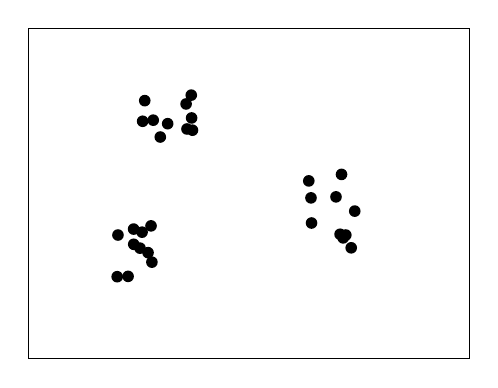
\begin{tikzpicture}[scale=1.4]
			\draw (-0.5,-0.4) rectangle (3.5,2.6);
			
			\fill (0.456,0.778)circle (1.5pt);
			\fill (0.622,0.478)circle (1.5pt);
			\fill (0.457,0.64)circle (1.5pt);
			\fill (0.614,0.807)circle (1.5pt);
			\fill (0.314,0.724)circle (1.5pt);
			\fill (0.533,0.75)circle (1.5pt);
			\fill (0.514,0.605)circle (1.5pt);
			\fill (0.307,0.346)circle (1.5pt);
			\fill (0.406,0.349)circle (1.5pt);
			\fill (0.587,0.564)circle (1.5pt);
			
			\fill (2.065,1.061)circle (1.5pt);
			\fill (2.045,1.215)circle (1.5pt);
			\fill (2.292,1.07)circle (1.5pt);
			\fill (2.381,0.724)circle (1.5pt);
			\fill (2.43,0.608)circle (1.5pt);
			\fill (2.342,1.274)circle (1.5pt);
			\fill (2.329,0.731)circle (1.5pt);
			\fill (2.462,0.941)circle (1.5pt);
			\fill (2.357,0.698)circle (1.5pt);
			\fill (2.07,0.833)circle (1.5pt);
			
			\fill (0.765,1.734)circle (1.5pt);
			\fill (0.557,1.943)circle (1.5pt);
			\fill (0.698,1.613)circle (1.5pt);
			\fill (0.634,1.766)circle (1.5pt);
			\fill (0.979,1.993)circle (1.5pt);
			\fill (0.99 ,1.675)circle (1.5pt);
			\fill (0.538,1.756)circle (1.5pt);
			\fill (0.932,1.913)circle (1.5pt);
			\fill (0.982,1.786)circle (1.5pt);
			\fill (0.94 ,1.686)circle (1.5pt);
		\end{tikzpicture}
		\caption*{\footnotesize Original Set}
		\label{fig:badrep}
	\end{minipage}
	\hspace{1cm}
	\begin{minipage}{0.4\linewidth}
		\centering
		\begin{tikzpicture}[scale=1.4]
		\draw (-0.5,-0.4) rectangle (3.5,2.6);
		
		\fill (0.765,1.734)circle (1.5pt);
		\fill (0.514,0.605)circle (1.5pt);
		\fill (2.292,1.07)circle (1.5pt);
		\end{tikzpicture}		
		\caption*{\footnotesize Representative Subset}
		\label{fig:goodrep}
	\end{minipage}
	\caption{Example of a Representative Set}
	\label{fig:rep}
\end{figure}

This thesis aims to research, develop, and analyse different algorithms to choose a representative subset of geographic points, whilst being able to dynamically change that set of points via zooming or panning over a geographic region containing a large amount of geographical data. In case the optimal solution algorithms prove to be too slow, heuristic approaches will be implemented. Heuristic algorithms will have their solution quality and speed benchmarked against implicit enumeration algorithms.
The algorithm or algorithms that are deemed the most suitable to solve the task will be integrated in a web framework via the \emph{geojson} and \emph{WFS} (web feature service) geographic data communication standards . Figure \ref{fig:arch} shows the basic concept of the architecture for the web application.

\begin{figure}[H]
	\begin{center}
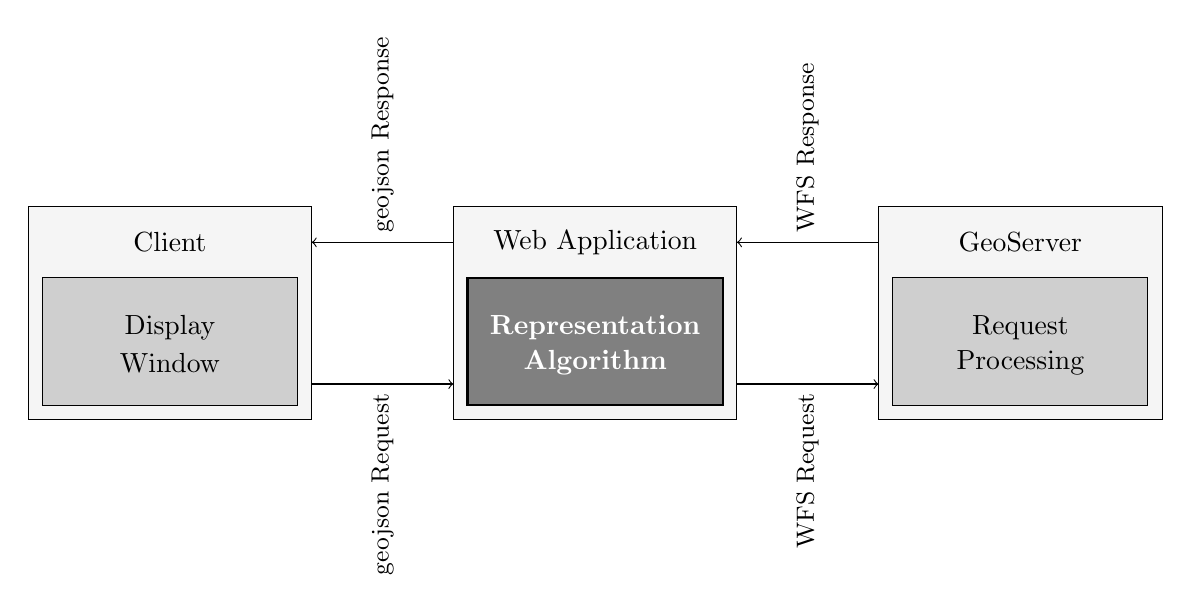
\begin{tikzpicture}[scale=0.9]
	\begin{scope}[]
		\fill[lightgray!15,draw=black] (0,0) rectangle (4,3);
		\fill[lightgray!75,draw=black] (0.2,0.2) rectangle (3.8,2);
		\node at (2,2.5) {Client};
		\node at (2,1.3) {Display};
		\node at (2,0.8) {Window};
	\end{scope}
	\begin{scope}[shift={(6,0)}]
		\fill[lightgray!15,draw=black] (0,0) rectangle (4,3);
		\fill[black!50,draw=black,thick] (0.2,0.2) rectangle (3.8,2);
		\node at (2,2.5) {Web Application};
		\node[text=white] at (2,1.3) {\textbf{Representation}};
		\node[text=white] at (2,0.8) {\textbf{Algorithm}};
	\end{scope}
	\begin{scope}[shift={(12,0)}]
		\fill[lightgray!15,draw=black] (0,0) rectangle (4,3);
		\fill[lightgray!75,draw=black] (0.2,0.2) rectangle (3.8,2);
		\node at (2,1.3) {Request};
		\node at (2,0.8) {Processing};
		\node at (2,2.5) {GeoServer};
	\end{scope}
	
	\begin{scope}[shift={(6,-0.5)},rotate=90]
		\draw[->] (1,2) -- node[left,rotate=90] {\small geojson Request} (1,0) ;
		\draw[<-] (3,2) -- node[right,rotate=90] {\small geojson Response} (3,0);
	\end{scope}


	\begin{scope}[shift={(12,-0.5)},rotate=90]
		\draw[->] (1,2) -- node[left,rotate=90] {\small WFS Request} (1,0) ;
		\draw[<-] (3,2) -- node[right,rotate=90] {\small WFS Response} (3,0);
	\end{scope}
\end{tikzpicture}
\end{center}
\caption{Proposed Program Architecture}
\label{fig:arch}
\end{figure}

The application is meant to function as an independent module capable of being decoupled and used for different clients and/or servers, should the need arise in the future.

Some famous web applications and services perform similar operations that already select from large sets of points. Most of these rely on having different preprocessed layers of information, which contain similarly ranked points. For example, a map of a continent would only request the layer containing the capitals of the visible countries, whilst a map of a singular country would only request the layer containing the cities within the viewing window's coordinates.

This solution requires that a lot of preprocessed data be stored in a fairly large and robust database. It also skips the representation problem by having points with different importance ranks. If any geographic query returns too many points for the application to render, then it could choose to only display the higher ranked ones or, alternatively, repeat the same query to the layer above to reduce the stress. Since this problem requires that no storage space is used, other solutions must be found.

Another approach is done by projecting all points to a limited resolution image format. Mapping vectorial points into a bitmap format with no aliasing means that all points that are closer together than a pixel will likely be rounded off to the same spot, effectively merging the two points.

Explicitly creating an image file may result in a larger file, which may cause problems in a bandwidth-dependant web application. The solution to this would be to round the coordinates of every point to a grid, and only relay the coordinates of the grid that would contain any points. This method, however, would mean a loss of precision increasing with the size of the grid. Furthermore, the points selected would be grid-aligned, and not necessarily correspond with any of the original, vectorial set. This would make for a visual pattern, which would be obvious for a human user. This solution is therefore also not suitable for our purpose.

Since no suitable algorithms were found, new ones had to be designed to properly solve the problem. The first approach interpreted the representation problem as an optimization problem known as \emph{Minimum Coverage Subset}. This problem requires that a number of points is chosen out of the original set to become the representative set. It finds the best possible combination of the original set such points to represent it, with the cardinality constrained to an input value. This constrain meant that the number of representative points must be known before the algorithm is executed, which is not always the case. Because of this particular limitation, and coupled with performance issues, a second approach was made. In this new approach, the algorithm is given a minimum distance between points in the representative set. The algorithm must then find the smallest collection of circles with this distance as their radius such that no point in the set is uncovered. This is known as a \emph{Geometric Disk Cover} problem, and our specific formulation has one extra constraint that makes it so that the circles need to have their centres on points of the original set. Because of the performance issues met in the first approach, this problem was solved using an approximation algorithm, which compromises the quality of the result (within a controlled threshold) in order to be performed in a more reasonable time. 

This report is organized as follows:
Chapter \ref{chap:theory} - \nameref{chap:theory} defines the base theoretical concepts, such as a notion of representativeness, as well as some useful structures used in the algorithms. Chapter \ref{chap:algos} - \nameref{chap:algos} describes the implicit enumeration algorithms implemented for the minimum coverage set problem, as well as an analysis on their time and space complexities. Chapter \ref{chap:approx} - \nameref{chap:approx} describes the approximation algorithm for the geometric disk coverage problem, as well as heuristic accelerations and a space and time complexity analysis. The chapter ends with a proposed solution to the issue of panning the viewing window.